\documentclass[12pt,titlepage]{article}
\usepackage[margin=1.25in]{geometry}
\usepackage{graphicx,amsmath,blindtext,minted}

%% Variables definition
\newcommand{\vSubject}{Mathematics 3}
\newcommand{\vSubtitle}{Scalar and Vector}
\newcommand{\vName}{Muhammad Baihaqi Aulia Asy'ari}
\newcommand{\vNIM}{2241720145}
\newcommand{\vClass}{2I}
\newcommand{\vDepartment}{Information Technology}
\newcommand{\vStudyProgram}{D4 Informatics Engineering}

%% [START] Tikz related stuff
\usepackage{tikz}
\usetikzlibrary{svg.path,calc,shapes.geometric,shapes.misc}
\tikzstyle{terminator} = [rectangle, draw, text centered, rounded corners = 1em, minimum height=2em]
\tikzstyle{preparation} = [chamfered rectangle, chamfered rectangle sep=0.75em, draw, text centered, minimum height = 2em]
\tikzstyle{process} = [rectangle, draw, text centered, minimum height=2em]
\tikzstyle{decision} = [diamond, aspect=2, draw, text centered, minimum height=2em]
\tikzstyle{data}=[trapezium, draw, text centered, trapezium left angle=60, trapezium right angle=120, minimum height=2em]
\tikzstyle{connector} = [line width=0.25mm,->]
%% [END] Tikz related stuff

%% [START] Fancy header related stuff
\usepackage{fancyhdr}
\pagestyle{fancy}
\setlength{\headheight}{15pt} % compensate fancyhdr style
\fancyhead{}
\fancyfoot{}
\fancyfoot[L]{\thepage}
\fancyfoot[R]{\textit{\vSubject - \vSubtitle}}
\renewcommand{\footrulewidth}{0.4pt}% default is 0pt, overline for footer
%% [END] Fancy header related stuff

%% [START] Custom tabular command related stuff
\usepackage{tabularx}
\newcommand{\details}[2]{
    #1 & #2  \\
}
%% [END] Custom tabular command related stuff

%% [START] Figure related stuff
\newcommand{\image}[3][1]{
    \begin{figure}[h]
        \centering
        \includegraphics[#1]{#2}
        \caption{#3}
        \label{#3}
    \end{figure}
}
%% [END] Figure related stuff

%%
\usepackage{pgf-umlcd}

\renewcommand{\umldrawcolor}{black}
\renewcommand{\umlfillcolor}{white}
%%

%% [BEGIN] Custom enumerator
\usepackage{enumitem}
%% [END] Custom enumerator

%% [BEGIN] Paragraph indent
\usepackage{indentfirst}
%% [END] Paragraph indent

\begin{document}
\begin{titlepage}
    \centering
    \vfill
    {\bfseries\LARGE
        \vSubject\\
        \vskip0.25cm
        \vSubtitle
    }
    \vfill
    
\includegraphics[width=6cm]{images/polinema-logo.png}
    \vfill
    {
        \textbf{Name}\\
        \vName\\
        \vskip0.5cm
        \textbf{NIM}\\
        \vNIM\\
        \vskip0.5cm
        \textbf{Class}\\
        \vClass\\
        \vskip0.5cm
        \textbf{Department}\\
        \vDepartment\\
        \vskip0.5cm
        \textbf{Study Program}\\
        \vStudyProgram
    }
\end{titlepage}

\newpage

\section*{Exercise 1}
\begin{enumerate}
    \item Scalar
    \item Vector
    \item Scalar
    \item Scalar
\end{enumerate}

\section*{Exercise 2}
\begin{center}
    \includegraphics[width=.6\textwidth]{images/figures/fig1.png}
\end{center}
x is the equivalent of a Vector and A is the equivalent of a Matrix. A\textunderscore t variable is a transposed A variable. the A\textunderscore t.shape shows what the ordo of the Matrix A after getting transposed.
\section*{Exercise 3}
\begin{center}
    \includegraphics[width=.6\textwidth]{images/figures/fig2.png}
\end{center}
the row vector is just a standart array. the column vector is technically a 2D array with only 1 column and thus creating a vector that's presented in a column.
\section*{Exercise 4}
\begin{center}
    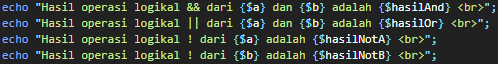
\includegraphics[width=.6\textwidth]{images/figures/fig3.png}
\end{center}
the vector[2] select the 3 element of the vector. 
\begin{center}
    \includegraphics[width=.6\textwidth]{images/figures/fig4.png}
\end{center}
the vector[:] select all element, vector[:3] select first 3 element, vector[3:] select every element past the 3rd element.
\section*{Exercise 5}
There are many operation we can do with vector and matrix and n-dimensional array
\section*{Exercise 6}
Vectors are used in listing things and matrixes are used in making tables

\end{document}